\let\negmedspace\undefined
\let\negthickspace\undefined
\documentclass[journal]{IEEEtran}
\usepackage[a4paper, margin=10mm, onecolumn]{geometry}
%\usepackage{lmodern} % Ensure lmodern is loaded for pdflatex
\usepackage{tfrupee} % Include tfrupee package

\setlength{\headheight}{1cm} % Set the height of the header box
\setlength{\headsep}{0mm}  % Set the distance between the header box and the top of the text

\usepackage{gvv-book}
\usepackage{gvv}
\usepackage{cite}
\usepackage{amsmath,amssymb,amsfonts,amsthm}
\usepackage{algorithmic}
\usepackage{graphicx}
\usepackage{float}
\usepackage{textcomp}
\usepackage{xcolor}
\usepackage{txfonts}
\usepackage{listings}
\usepackage{enumitem}
\usepackage{mathtools}
\usepackage{gensymb}
\usepackage{comment}
\usepackage[breaklinks=true]{hyperref}
\usepackage{tkz-euclide} 
\usepackage{listings}
% \usepackage{gvv}                                        
\def\inputGnumericTable{}                                 
\usepackage[latin1]{inputenc}                                
\usepackage{color}                                            
\usepackage{array}                                            
\usepackage{longtable}                                       
\usepackage{calc}                                             
\usepackage{multirow}                                         
\usepackage{hhline}                                           
\usepackage{ifthen}                                           
\usepackage{lscape}
\usepackage{tikz}
\usetikzlibrary{patterns}

\begin{document}

\bibliographystyle{IEEEtran}
\vspace{3cm}

\title{3.2.4}
\author{ee25btech11063-vejith}

\maketitle
% \maketitle
% \newpage
% \bigskip
{\let\newpage\relax\maketitle}
\renewcommand{\thefigure}{\theenumi}
\renewcommand{\thetable}{\theenumi}
\setlength{\intextsep}{10pt} % Space between text and floats
\textbf{Question}:\\
Construct the triangle BD$^{\prime}$C$^{\prime}$ similar to $\triangle$BDC with scale factor $\frac{4}{3}$.Draw the line segment D$^{\prime}$A$^{\prime}$ parallel to DA where A$^p$rime lies on extended side BA.Is A$^{\prime}$BC$^{\prime}$D$^{\prime}$ a parallelogram?\\ 
\textbf{solution}
\begin{table}[h!]    
  \centering
  \begin{tabular}[12pt]{ |c| c|}
    \hline
      \textbf{Vector} & \textbf{Name}\\ 
      \hline
      \myvec{0\\0} & Vector $\Vec{A}$\\
      \hline
      \myvec{4\\0} & Vector $\Vec{B}$\\
      \hline
      \myvec{4\\3} & Vector $\Vec{C}$\\
      \hline
      \myvec{0\\3} &  Vector $\Vec{D}$\\
      \hline
      \end{tabular}
  \caption{Variables Used}
  \label{}
\end{table}\\
consider $\triangle$BDC.constructs a $\triangle$BD$^{\prime}C^{\prime}$
 with scale factor $\frac{4}{3}$.\\
This means 
\begin{align}
  \triangle BD^{\prime}C^{\prime} \sim \triangle BDC.\\
\frac{\norm{\vec{D^{\prime}}-\vec{B}}}{\norm{\vec{D}-\vec{B}}} \;=\; \frac{\norm{\vec{C^{\prime}}-\vec{B}}}{\norm{\vec{C}-\vec{B}}} \;=\; \frac{\norm{\vec{C^{\prime}}-\vec{D^{\prime}}}}{\norm{\vec{C}-\vec{D}}} \;=\; \frac{4}{3}.\\
\Vec{D^{\prime}}=\Vec{B}+\frac{4}{3}(\Vec{D}-\Vec{B})\\
\Vec{D^{\prime}}=\myvec{-4/3\\4}\\
\Vec{C^{\prime}}=\Vec{B}+\frac{4}{3}(\Vec{C}-\Vec{B})\\
\Vec{C^{\prime}}=\myvec{4\\4}
\end{align}

\textbf{Construct A$^{\prime}$}\\
Mark $\vec{D^{\prime}}$ and $\vec{A^{\prime}}$ parallel to $\vec{D}-\vec{A}$ with $\vec{A^{\prime}}$ along the direction of  $\vec{B}-\vec{A}$.\\
\begin{align}
\vec{A^{\prime}-D^{\prime}}=\lambda(\vec{A}-\vec{D})\\
\vec{A^{\prime}}=\myvec{-4/3\\4}+\lambda(\myvec{0\\-3})\\
\implies \vec{A^{\prime}}=\myvec{-4/3\\4-3\lambda}
\end{align}
 $\vec{A^{\prime}}$ lies on line through $\vec{B}-\vec{A}$ so,
 \begin{align}
 \vec{A^{\prime}}=\vec{B}+\mu(\vec{A}-\vec{B})\\
 \implies \vec{A^{\prime}}=\myvec{-4\mu\\0}\\
 \end{align}
 From equation (9) and (11)
 \begin{align}
 \lambda=4/3 \text{and} \mu=1/3\\
 \implies \vec{A^{\prime}}=\myvec{-4/3\\0}\\
    \Vec{B}-\Vec{A}=\myvec{4\\0}-\myvec{0\\0}=\myvec{4\\0}\\
    \Vec{C}-\Vec{D}=\myvec{4\\3}-\myvec{0\\3}=\myvec{4\\0}\\
\implies \Vec{B}-\Vec{A}=\Vec{C}-\Vec{D}
\end{align}

\textbf{Check the parallelogram property of A$^{\prime}$BC$^{\prime}$D$^{\prime}$ }\\
\begin{align}
    \vec{B}-\vec{A^{\prime}}=-t(\vec{A}-\vec{B})\\
    \vec{D^{\prime}}-\vec{C^{\prime}}=k(\vec{C}-\vec{D})\\
    \text{From Equation (17) }\Vec{B}-\Vec{A}=\Vec{C}-\Vec{D}\\
\implies \vec{B}-\vec{A^{\prime}}=-t(\vec{A}-\vec{B})=t(\vec{C}-\vec{D})=\frac{t}{k}\vec{D^{\prime}}-\vec{C^{\prime}}\\
\implies \vec{B}-\vec{A^{\prime}} \parallel \vec{D^{\prime}}-\vec{C^{\prime}}
\end{align}
\text{By construction of A$^{\prime}$} 
    \begin{align}
    \vec{D^{\prime}}-\vec{A^{\prime}} \parallel \vec{D}-\vec{A}\\
    \vec{D}-\vec{A} \parallel \Vec{C}-\vec{B}\\
     \Vec{C}-\vec{B} \parallel \Vec{C^{\prime}}-\Vec{B}\\
\implies \vec{D^{\prime}}-\vec{A^{\prime}} \parallel \Vec{C^{\prime}}-\Vec{B}
\end{align}
$\implies$A$^{\prime}$BC$^{\prime}$D$^{\prime}$ a parallelogram
\begin{figure}[H]
    \centering
    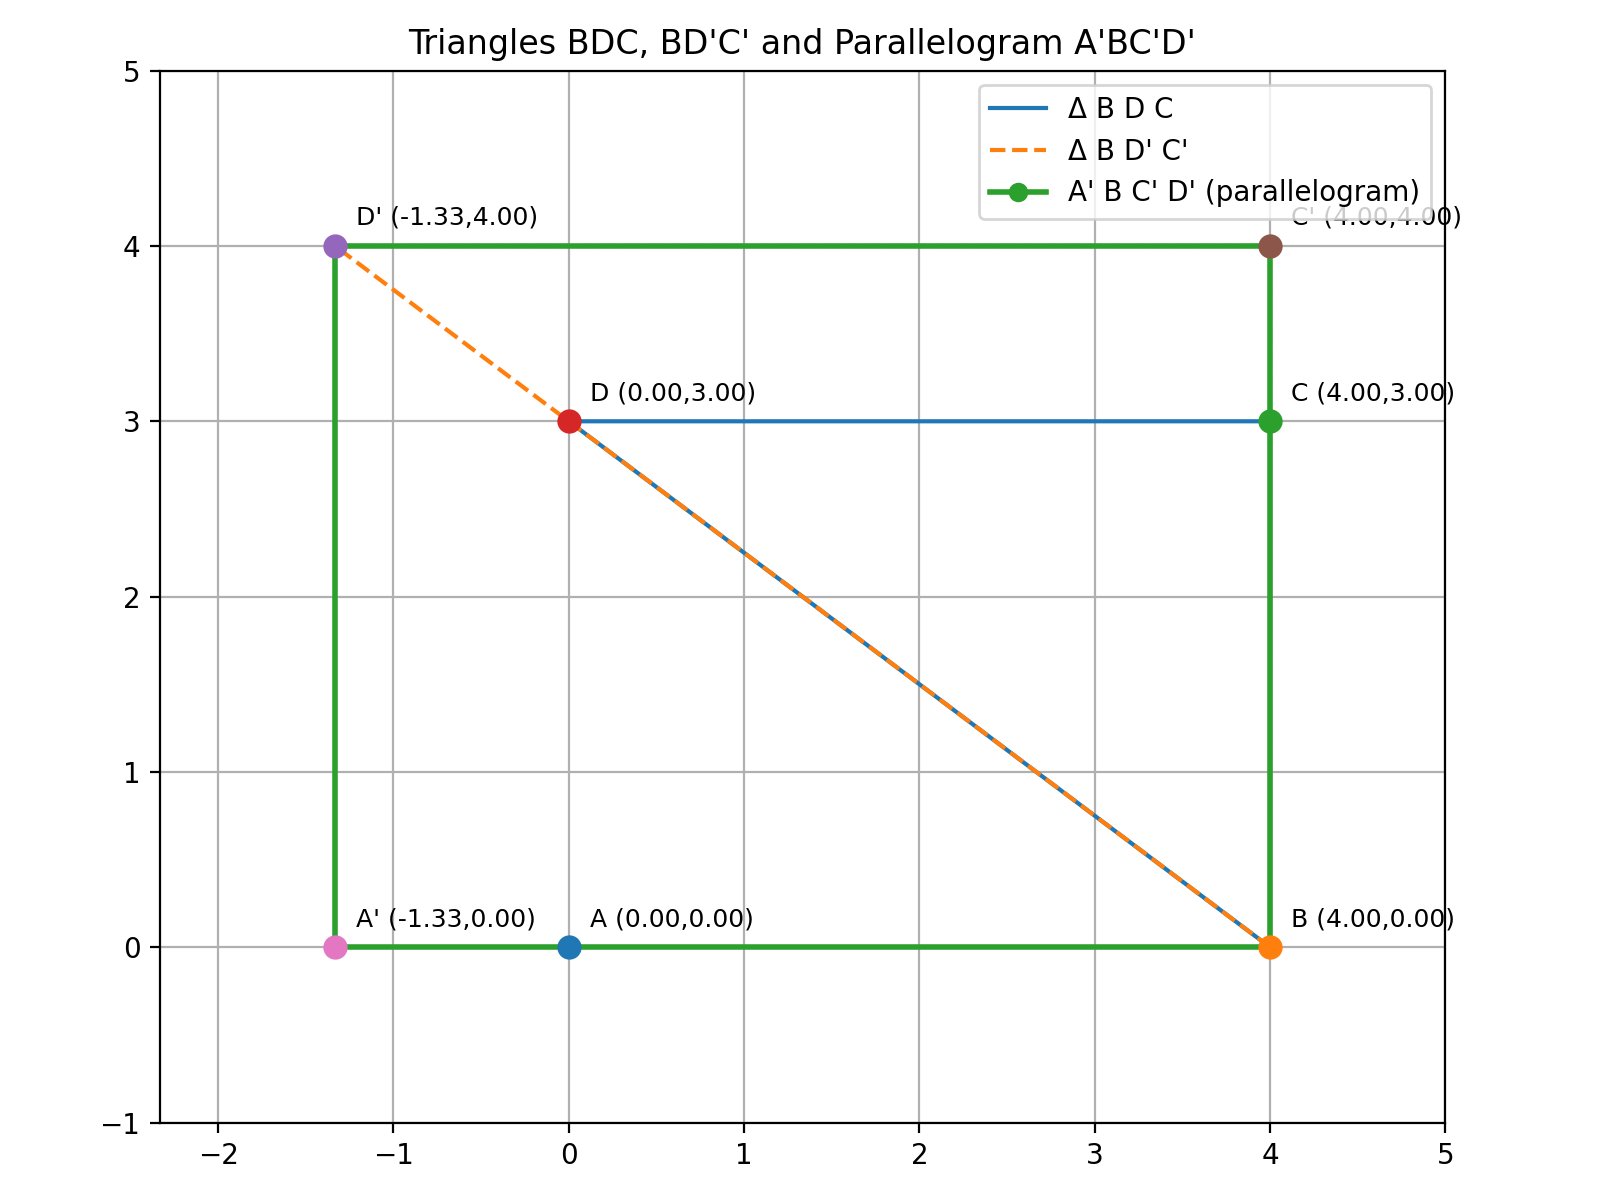
\includegraphics[width=1.0\columnwidth]{figs/01.png}
    \label{fig-1}
\end{figure}
\end{document}




